% !TEX root = research_report.tex
%上の記述は消さないこと.章(分割ファイル)を増やしたときも忘れずに記述する.
\chapter{理論}
ここの部分にはこの章の概要を記述する.

\section{○○制御理論}

ありがちなのが段落の作り忘れ.以下のように空行を入れると自動的に段落が作成される.

テストテストテストテストテストテストテストテストテストテストテストテストテストテストテストテス
トテストテストテストテストテストテストテストテスト



\section{図表の貼り付け}
表を示したときは必ず参照する.表\ref{t1}のように・・・
\begin{table}[htbp]
\caption{表}
\label{t1}
\begin{center}
  \begin{tabular}[tb]{|c|c|c|c|c|c|c|c|c|}
   \hline
  aa & bb& cc & aa & bb& cc & aa & bb& cc \\ \hline
  aa & bb& cc & aa & bb& cc & aa & bb& cc \\ \hline
  aa & bb& cc & aa & bb& cc & aa & bb& cc \\ \hline
  aa & bb& cc & aa & bb& cc & aa & bb& cc  \\ \hline
  aa & bb& cc & aa & bb& cc & aa & bb& cc \\ \hline
 \end{tabular}
\end{center}
\end{table}

報告書では領域をケチらず,図は大きく貼り付けること.そして,貼り付けた図は表と同様に必ず本文中で
参照する.図\ref{amp}に示すように・・・.
\begin{figure}[htbp]
 \begin{center}
  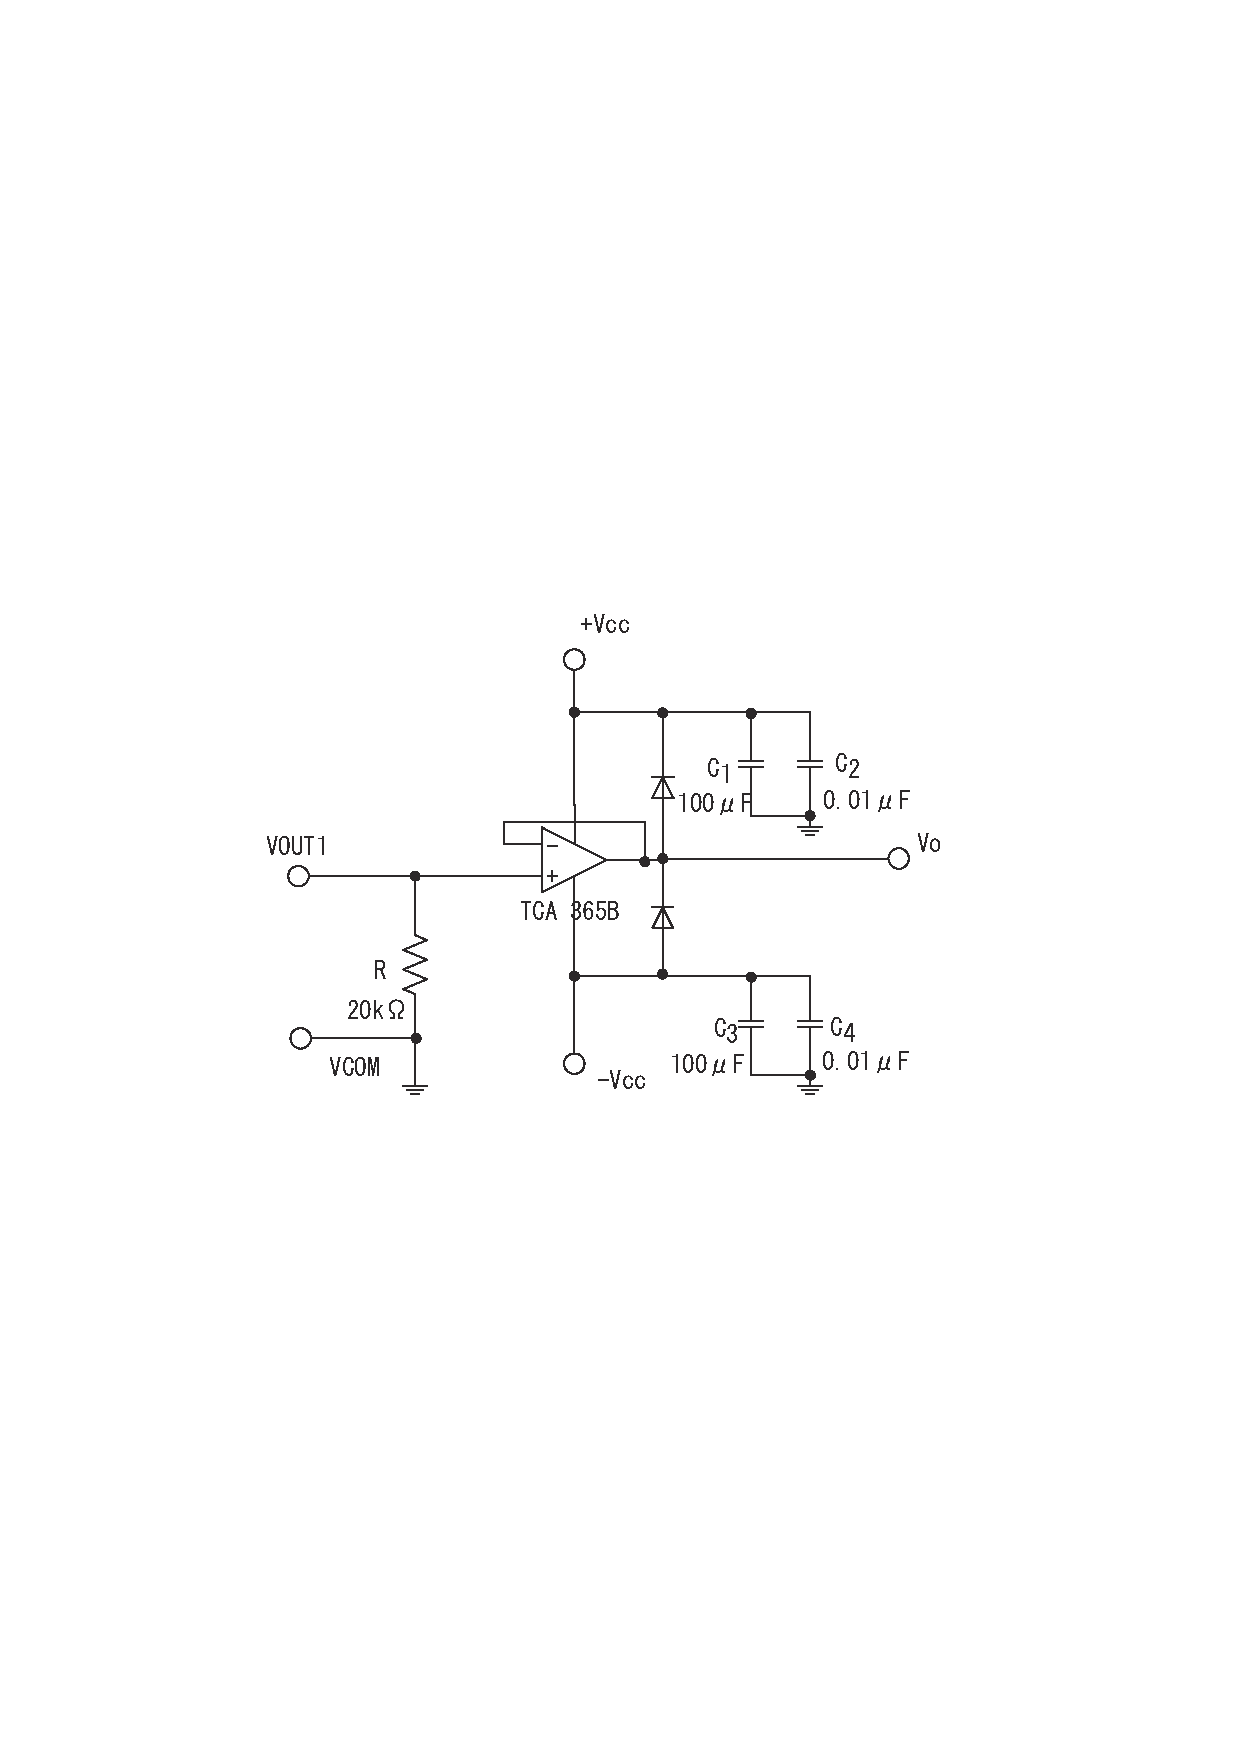
\includegraphics[width = 14.0cm]{./fig/drive_circuit.pdf}
 \end{center}
 \caption{オペアンプ回路図}
 \label{amp}
\end{figure}

これが\TeX のよいところ.図表の位置を変えても自動的に図番号が変化する.

\section{数式}
1行で収まる数式
\begin{equation}
 \int_0^\infty \frac{\sin x}{\sqrt{x}} dx = \sqrt{\frac{\pi}{2}}\label{eq1}
\end{equation}

複数行にわたる数式
\begin{eqnarray}
 \bm{\dot x}&=&\bm{Ax}+\bm{Bu}\label{eq2-1} \\
 \bm{y}&=&\bm{Cx}+\bm{Du}\label{eq2-2}
\end{eqnarray}

文中に数式を入れることも可能$F=m\alpha$である.ただし式番号はつかない.

行列
\begin{equation}
 \begin{bmatrix} 
  A & B & C\\ 
  D & E & F 
 \end{bmatrix}
\end{equation}

ギリシャ文字は数式環境で記述する.\underline{全角で書かない!}

$\alpha,\beta,\gamma,\Gamma,\delta,\Delta,\omega,\Omega,\varepsilon$

必要であれば,式(\ref{eq1}),式(\ref{eq2-1}),式(\ref{eq2-2})のように参照する.

ちなみに,単位はイタリックにしない.$\theta=\frac{\pi}{2}[\mathrm{rad}]$とする.
